\textbf{{1. 传输层的服务介绍}}

{{传输层提供了两种类型的服务:}}\textbf{{无连接服务和面向连接服务。}}{相应的实现分别是\textbf{用户数据报协议(UDP)和传输控制协议(TCP)}。当采用TCP时,传输层向上提供的是一条全双工的可靠的逻辑信道;当采用UDP时,传输层向上提供的是一条不可靠的逻辑信道。}

\textbf{{2.UDP的主要特点}}

1)传送数据前无需建立连接,数据到达后也无需确认。

2)不可靠交付。

3)报文头部短,传输开销小,时延较短。

\textbf{{3.TCP的主要特点}}

1)面向连接,不提供广播或多播服务。

2)可靠交付。

3)报文段头部长,传输开销大。

\textbf{{4. UDP数据报与IP分组的区别}}

IP分组要经过互联网中许多路由器的存储转发,但UDP数据报是在传输层的端到端抽象的逻辑信道中传送的,\textbf{UDP数据报只是IP数据报中的数据部分}(见下图),对路由器是不可见的。

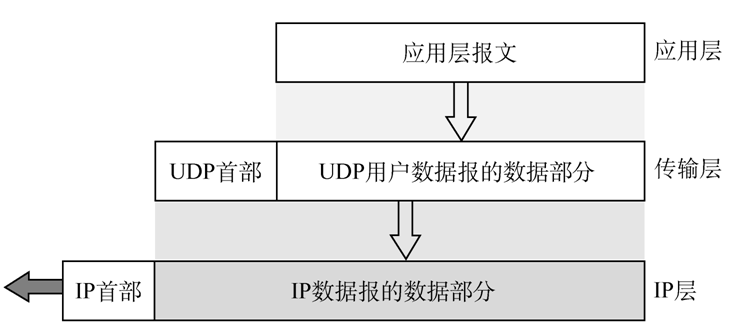
\includegraphics[width=3.33333in,height=1.53125in]{png-jpeg-pics/6AA6B83CA31AA36641EBBDBCB8F7FEA2.png}
